\subsection{Deep Learning for Pulse Shape Analysis with TRACE}
With the rise of user-friendly machine learning frameworks such as TensorFlow~\cite{tensorflow} or Pytorch~\cite{pytorch}, Deep Learning had seen a wide range of applications in physics~\cite{ml4phys}. In experimental nuclear and subnuclear physics pre-trained Neural Network (NN) can be used for task such as event tagging~\cite{baldi} or inside the trigger system/acquisition chain in HEP experiments~\cite{williams}. 


In this section an application of NNs to perform particle discrimination using the signals collected from the TRACE detector is presented. Such a technique can be used to improve data processing speed or even inside the acquisition system in future.
The code of the following analysis is available at~\cite{github-nn}.

\subsubsection{Dataset and training}

In order to train a network to discriminate between two different kinds of signals from the detector we need a dataset of labeled signals from the classes we want to distinguish. Data from the run \emph{25} are assigned to three different classes based on cuts made in the region of the graph in Fig.~\ref{imax}, either labeled as \emph{proton}, \emph{alpha} or \emph{other}, the dataset is then balanced resulting in \num{39000} labeled input signals to train the network, \num{13000} for each class. Examples of signals are shown in Fig.~\ref{input}.

\begin{figure}[htb]
  \centering
  \begin{minipage}[b]{0.45\textwidth}
    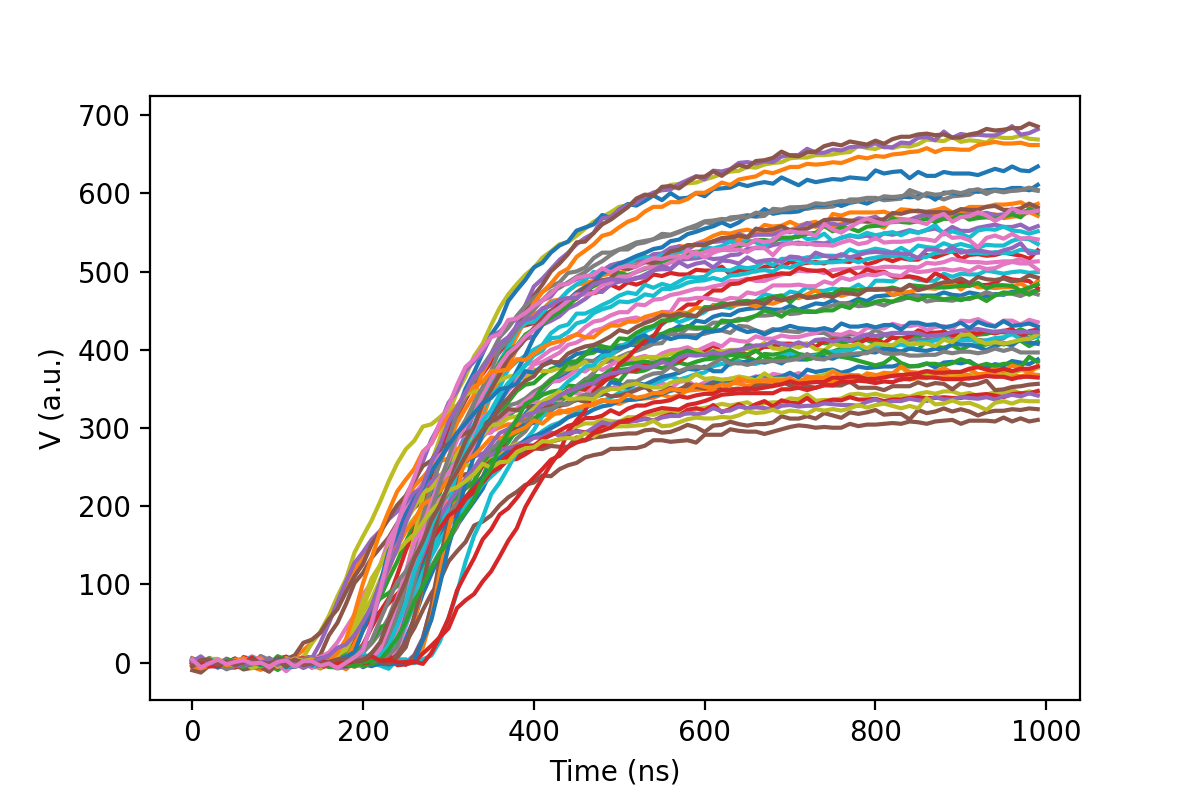
\includegraphics[width=\textwidth]{img/protons.png}
    \caption{Protons}
    %\label{}
  \end{minipage}
  \hfill
  \begin{minipage}[b]{0.45\textwidth}
   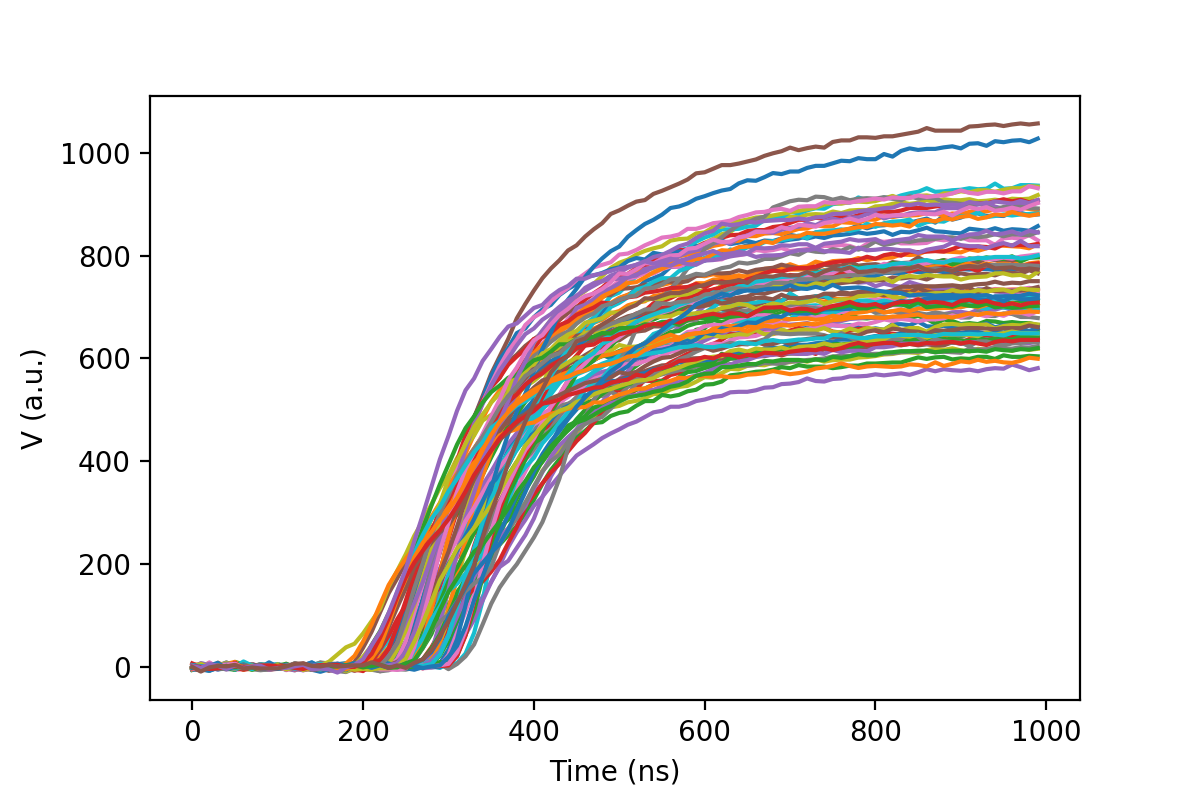
\includegraphics[width=\textwidth]{img/alpha.png}
  \caption{Alpha}
  %\label{}
  \end{minipage}
  \hfill
  \begin{minipage}[b]{0.45\textwidth}
   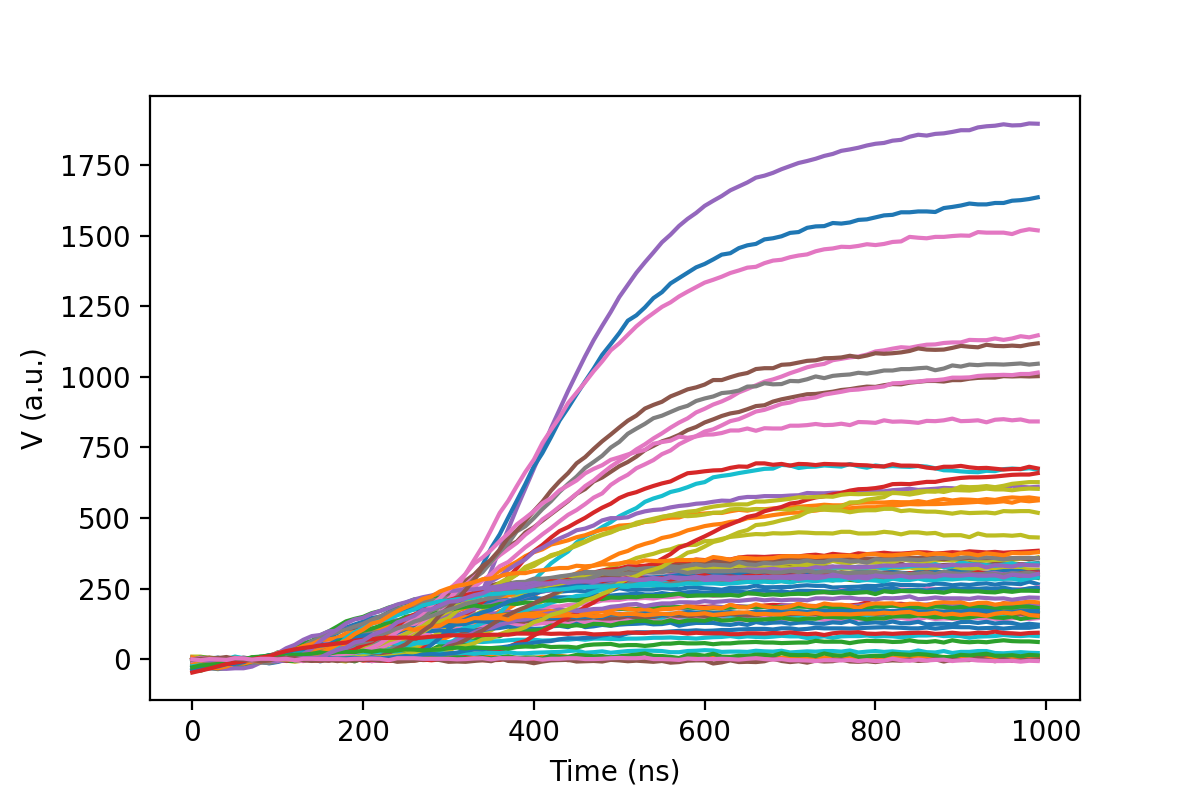
\includegraphics[width=\textwidth]{img/other.png}
  \caption{Other}
  %\label{}
  \end{minipage}
  \caption{Examples of input from the three classes.}
  \label{input}
\end{figure}

The dataset is split into the actual training data (\num{90}\%) and a set for validation (\num{10}\%). The training data are then fed to a simple feedforward NN istantiated into the framework Pytorch with the following architecture:

\begin{itemize}
	\item Input layer (The \num{100} points of the sampled signal)
	\item 2 Hidden layers of 64 units (\emph{ReLU} activation)
	\item Output layer (\emph{softmax} activation, 3 classes).
\end{itemize}

The training is performed optimizing a Mean Squared Error (MSE) function for the labels using the \emph{Adamax} optimizer. Data are given in batches of 200 samples, over several ($\sim 30$) epochs of training. At the end is possible use the model on data from other run to classify events from other run.

\subsubsection{Validation and Application of the model}

The perfomance of the network is evaluated using both the validation dataset of \num{3900} samples not used for the training and a dataset of 2960 events taken from one calibration run using an alpha source.


The maximal accuracy (percentage of events classified correctly) achievable on the testing dataset is of $\sim\num{94} \%$ with the confusion matrix shown in Fig.~\ref{conf_test}, which shows that overall no bias is present on the misclassified events.


Using the data from the calibration run an accuracy of $\sim\num{67} \%$ is achieved which is significantly lower from the former result, this is exected due to the fact that the data are taken in different condition, nonetheless the confusion matrix in Fig.~\ref{conf_alpha} shows that the NN almost never missclassify an alpha particle for a proton.

\begin{figure}[htb]
  \centering
  \begin{minipage}[b]{0.45\textwidth}
    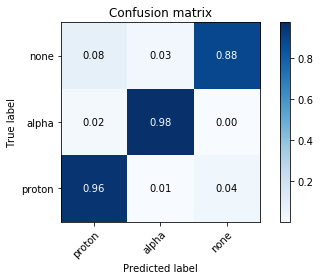
\includegraphics[width=\textwidth]{img/conf_test.png}
    \caption{Test dataset}
    \label{conf_test}
  \end{minipage}
  \hfill
  \begin{minipage}[b]{0.45\textwidth}
   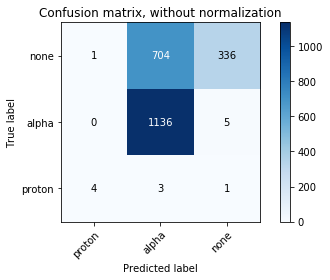
\includegraphics[width=\textwidth]{img/conf_alphas.png}
  \caption{Calibration Run}
  \label{conf_alpha}
  \end{minipage}
  \caption{Confusion matrices for the two datasets.}
  \label{input}
\end{figure}

At the end of the validation the trained model is exported and implemented into a C++ program that merges the data of the previous trees with the output of the neural network, this two new entries should be interpreted as probabilities of the particle being an proton or alpha in the energy range of the particles which stop into the $\Delta E$ detector (below $\sim \num{4}/\num{6}$ MeV). 

The final ROOT TTree is complete of the data from the GALILEO detector array and can be used to look for coincidence between the emitted particles from the compounds formed and $\gamma$'s emitted from the disexcitation of the resulting nuclei.





